\documentclass[10pt,twocolumn]{extarticle}
\usepackage[a4paper,margin=1.5cm,columnsep=0.7cm]{geometry}
\usepackage{amsmath,amssymb}
\usepackage{graphicx}
\usepackage{enumitem}
\usepackage{booktabs}
\usepackage{array}
\usepackage{tabularx}
\usepackage[T1]{fontenc}

\setlength{\parindent}{0pt}
\setlength{\parskip}{4pt}
\renewcommand{\arraystretch}{1.15}

\newenvironment{qoptions}{\begin{itemize}[leftmargin=1.8em,itemsep=2pt,topsep=2pt,label={}]}{\end{itemize}}
\newcommand{\opt}[2]{\item[({#1})] {#2}}

\newcommand{\sectionhdr}[1]{\par\vspace{4pt}\noindent\textbf{\large #1}\par\vspace{2pt}}
\newcommand{\subsectionhdr}[1]{\par\vspace{3pt}\noindent\textbf{#1}\par\vspace{2pt}}

\pagestyle{empty}

\begin{document}
\twocolumn[
\begin{center}
{\LARGE\bfseries JEE (Main+Advanced) Score-II --- Test 29 (26 Mar 2024)}
\end{center}
\vspace{6pt}
]

\sectionhdr{PART-1: PHYSICS}
\subsectionhdr{Section-I (i): Single Correct}

\textbf{1.} Three charges q, q and $-2q$ are fixed on the vertices of an equilateral triangular insulated plate of edge length a. This plate is in equilibrium between two very large plates having surface charge density $\sigma_1$ and $\sigma_2$ respectively. Find the period of small angular oscillation about an axis passing through its centroid and perpendicular to plane. Moment of inertia of the system about this axis I. (Neglect gravity)

\begin{qoptions}
\opt{A}{$2\pi\sqrt{\dfrac{\varepsilon_0 I}{qa|\sigma_1-\sigma_2|}}$}
\opt{B}{$2\pi\sqrt{\dfrac{\varepsilon_0 I}{2qa|\sigma_1-\sigma_2|}}$}
\opt{C}{$2\pi\sqrt{\dfrac{2\varepsilon_0 I}{\sqrt3\,qa|\sigma_1-\sigma_2|}}$}
\opt{D}{$2\pi\sqrt{\dfrac{2\varepsilon_0 I}{qa|\sigma_1-\sigma_2|}}$}
\end{qoptions}

\textbf{2.} Six resistor, each of resistance R, are connected at their ends so as form tetrahedral frame. Now two cells of negligible internal resistance, and emf E is connected to the combination. One cell between any two corners and other cell between rest two corners. Thermal power developed will be:-

\begin{qoptions}
\opt{A}{$\dfrac{E^2}{R}$}
\opt{B}{$\dfrac{2E^2}{R}$}
\opt{C}{$\dfrac{4E^2}{R}$}
\opt{D}{$\dfrac{8E^2}{R}$}
\end{qoptions}

\textbf{3.} In a young's double slit interference experiment, the fringe pattern is observed on a screen placed at a distance D. The slits are separated by d ($\ll$ D) and are illuminated by coherent sources. The central maxima is formed at the geometrical centre on the screen with respect to the slits. If at a distance h from the central maximum on the screen the intensity is half of the maximum intensity then the value of $\lambda$ may be

\begin{qoptions}
\opt{A}{$\dfrac{2hd}{3D}$}
\opt{B}{$\dfrac{8hd}{19D}$}
\opt{C}{$\dfrac{4hd}{13D}$}
\opt{D}{$\dfrac{6hd}{11D}$}
\end{qoptions}

\textbf{4.} Ideal gas is in the container with a piston as one of the walls. There is a little hole in the wall opposite to piston, through which gas leaks out of the container at a rate R (number of molecules escaping the container per second). Now the gas is heated as well as compressed such that its temperature becomes 4 times its previous value, and pressure becomes 8 times its previous value. Now the rate of the gas out flow will be:

\begin{qoptions}
\opt{A}{2R}
\opt{B}{4R}
\opt{C}{8R}
\opt{D}{16R}
\end{qoptions}

\subsectionhdr{Section-I (ii): One or more correct}

\textbf{5.} A parallel plate capacitor is made of square conducting plates of side a and the separation between plates is d. The capacitor is connected with battery of emf V volt as shown in the figure.

\begin{center}
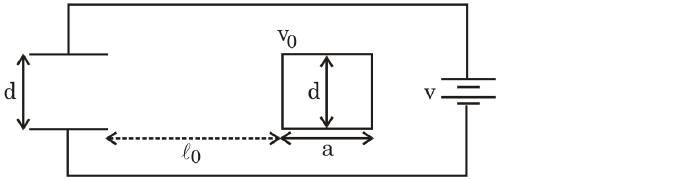
\includegraphics[width=0.9\linewidth]{Score-II - Test 29 (26 Mar 2024)-img/p1phy_q5_capacitor.png}
\end{center}

There is a dielectric slab of dimension $a\times a\times d$ with dielectric constant k. At t = 0, dielectric slab is given velocity v$_0$ towards capacitor as shown in the figure. (Neglect the effect of gravity and electrostatic force acting on the dielectric when dielectric is out side of capacitor. Also ignore any type frictional force acting on the dielectric during its motion) let the x be the length dielectric inside the capacitor at t = t sec. [$\ell_0\gg$a]

\begin{qoptions}
\opt{A}{Motion of dielectric slab is periodic but not simple harmonic motion.}
\opt{B}{Motion of dielectric slab is simple harmonic motion.}
\opt{C}{At any time, the slope of graph of total energy verses x is twice the slope of graph of potential energy verses x.}
\opt{D}{The value of maximum energy stored in the system is $\dfrac12 mV_0^2+\dfrac{\varepsilon_0 a^2V^2}{2d}(2k-1)$}
\end{qoptions}

\textbf{6.} A wooden cubical block ABCDEFGO of mass m and side `a' is wrapped by a square wire loop of perimeter 4a at a/2 as shown. The current in the wire I. The whole system is placed on frictionless horizontal surface in a uniform magnetic field $\vec B=B_0\hat j$. In this situation, normal force between horizontal surface and block passes through a point at a distance x from centre. Select the correct statement(s).

\begin{center}
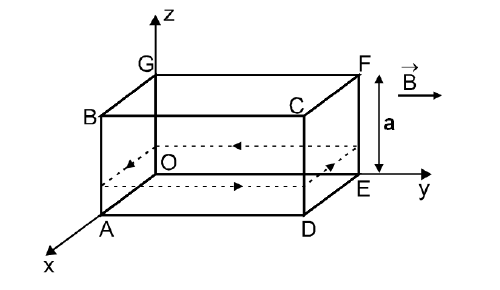
\includegraphics[width=0.7\linewidth]{Score-II - Test 29 (26 Mar 2024)-img/p1phy_q6_cube.png}
\end{center}

\begin{qoptions}
\opt{A}{The block must not topple if $I<\dfrac{mg}{aB_0}$}
\opt{B}{The block must not topple if $I<\dfrac{mg}{2aB_0}$}
\opt{C}{$x=\dfrac a4$ if $I=\dfrac{mg}{2aB_0}$}
\opt{D}{$x=\dfrac a4$ if $I=\dfrac{mg}{4aB_0}$}
\end{qoptions}

\textbf{7.} In space, there are 2 converging lens, whose optical axes coincide. Their focal length and initial distance are indicated.

\begin{center}
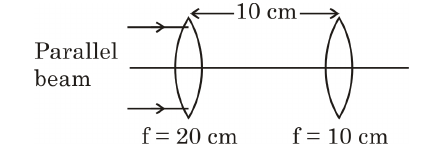
\includegraphics[width=0.65\linewidth]{Score-II - Test 29 (26 Mar 2024)-img/p1phy_q7_lens.png}
\end{center}

\begin{qoptions}
\opt{A}{If left lens only is moved to right, the final image moves to right.}
\opt{B}{If left lens only is moved to left, the final image moves to left.}
\opt{C}{If right lens only is moved to right, the final image moves to right.}
\opt{D}{If right lens only is moved to left, the final image moves to left.}
\end{qoptions}

\subsectionhdr{Section-I (iii): Matching List Sets}

\textbf{8.} There are some situation in List-I and in list-II time period of situation is given for small displacement. Match the list-I with list-II.

\textbf{List-I}

(P) A light rod attached to a particle of mass m

\begin{center}
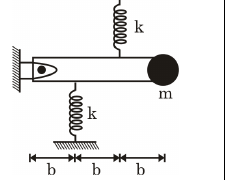
\includegraphics[width=0.55\linewidth]{Score-II - Test 29 (26 Mar 2024)-img/p1phy_q8_P.png}
\end{center}

(Q) Heavy rod and a particle of mass m each shown in figure. The particle is attached at other end of the rod

\begin{center}
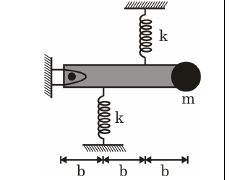
\includegraphics[width=0.55\linewidth]{Score-II - Test 29 (26 Mar 2024)-img/p1phy_q8_Q.png}
\end{center}

(R) A uniform rectangular plate having mass m

\begin{center}
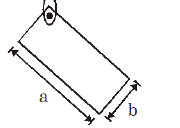
\includegraphics[width=0.4\linewidth]{Score-II - Test 29 (26 Mar 2024)-img/p1phy_q8_R.png}
\end{center}

(S) A uniform rectangular plate oscillate about an axis passing through O (mid point).

\begin{center}
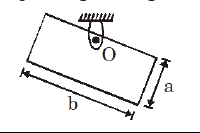
\includegraphics[width=0.4\linewidth]{Score-II - Test 29 (26 Mar 2024)-img/p1phy_q8_S.png}
\end{center}

\textbf{List-II}\\
(1) $4\pi\sqrt{\dfrac{3m}{5k}}$\quad (2) $6\pi\sqrt{\dfrac{m}{5k}}$\quad (3) $2\pi\sqrt{\dfrac{2\sqrt{a^2+b^2}}{3g}}$\quad (4) $2\pi\sqrt{\dfrac{a^2+4b^2}{6gb}}$\quad (5) $2\pi\sqrt{\dfrac{4a^2+b^2}{6ga}}$

\begin{qoptions}
\opt{A}{P $\to$ 2; Q $\to$ 1; R $\to$ 3; S $\to$ 5}
\opt{B}{P $\to$ 1; Q $\to$ 4; R $\to$ 5; S $\to$ 2}
\opt{C}{P $\to$ 3; Q $\to$ 2; R $\to$ 1; S $\to$ 4}
\opt{D}{P $\to$ 5; Q $\to$ 1; R $\to$ 2; S $\to$ 4}
\end{qoptions}

\textbf{9.} A steel rope (density d, length L, area of cross section A. Young's modulus Y) is subjected to operations as described in List-I. Discover the correct value of x in the expressions and match.

\textbf{List-I}

(P) The rope is hanging from a ceiling in equilibrium. The elastic potential energy per unit volume at a point L/3 from the ceiling is $\dfrac{x}{18}\dfrac{(dLg)^2}{Y}$

(Q) The rope is vertical and moves under the application of vertical force $F=\dfrac{dALg}{2}$ acting at its upper end upwards. The strain at a point at a distance $\dfrac L3$ from the lower end is $\dfrac{dLg}{xY}$

(R) The rope is rotating at angular speed $\omega_0$ in gravity free space about its one fixed end. The stress at a point $\dfrac L3$ from the fixed end is $\dfrac{x}{18}(dL^2\omega_0^2)$

(S) A circular ring is formed from the rope. This ring is made to rotate with angular speed $\omega_0$ in its own plane in gravity free space. Tension in the rope is x$\left(\dfrac{dAL^2\omega_0^2}{20\pi^2}\right)$

\textbf{List-II}\\
(1) 3\quad (2) 4\quad (3) 5\quad (4) 6\quad (5) None of these

\begin{qoptions}
\opt{A}{P $\to$ 4; Q $\to$ 2; R $\to$ 1; S $\to$ 5}
\opt{B}{P $\to$ 2; Q $\to$ 4; R $\to$ 5; S $\to$ 3}
\opt{C}{P $\to$ 1; Q $\to$ 3; R $\to$ 2; S $\to$ 4}
\opt{D}{P $\to$ 3; Q $\to$ 2; R $\to$ 4; S $\to$ 5}
\end{qoptions}

\textbf{10.} List-I indicated certain situations and list-II indicates the values of electric field (induced or electrostatic). Match the correct options:

\textbf{List-I}

(P) A uniformly charged solid infinite cylinder of radius R. x is distance from axis of cylinder

(Q) Current flowing through uniform cylindrical resistor. x is distance from left end. x is less than the length of resistor

\begin{center}
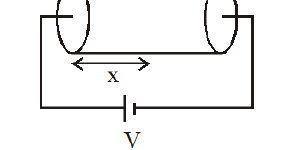
\includegraphics[width=0.75\linewidth]{Score-II - Test 29 (26 Mar 2024)-img/p1phy_q10_Q.png}
\end{center}

(R) An ideal solenoid of radius R. Current through solenoid is increasing with time. x is distance from axis of solenoid

\begin{center}
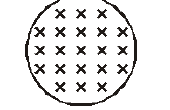
\includegraphics[width=0.3\linewidth]{Score-II - Test 29 (26 Mar 2024)-img/p1phy_q10_R.png}
\end{center}

(S) A conducting rod of length $\ell$ is moving in a direction perpendicular to the magnetic field with uniform velocity. x is distance from upper end. (x < $\ell$)

\begin{center}
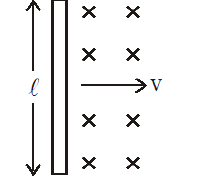
\includegraphics[width=0.35\linewidth]{Score-II - Test 29 (26 Mar 2024)-img/p1phy_q10_S.png}
\end{center}

\textbf{List-II}\\
(1) E = 0\quad (2) $|\vec E|$ increases with increase in x, reaches a maximum and then decreases.\quad (3) $|\vec E|$ decreases with increase in x, reaches a minimum and then increases.\quad (4) $|\vec E|$ is constant\quad (5) $|\vec E|$ continuously decreases with increase in x

\begin{qoptions}
\opt{A}{P $\to$ 3; Q $\to$ 1; R $\to$ 4; S $\to$ 5}
\opt{B}{P $\to$ 1; Q $\to$ 2; R $\to$ 3; S $\to$ 4}
\opt{C}{P $\to$ 4; Q $\to$ 5; R $\to$ 1; S $\to$ 2}
\opt{D}{P $\to$ 2; Q $\to$ 4; R $\to$ 2; S $\to$ 4}
\end{qoptions}

\textbf{11.} A uniform rod of mass m length $\ell$ is in a gravity free space and is free to move. An impulse J acts on the rod momentarily as shown in figure. Just after that moment.

\begin{center}
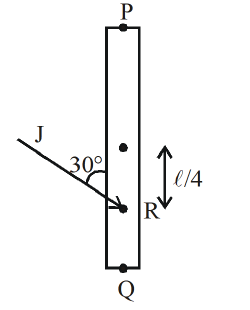
\includegraphics[width=0.4\linewidth]{Score-II - Test 29 (26 Mar 2024)-img/p1phy_q11_rod.png}
\end{center}

\textbf{List-I}\\
(P) Speed of upper end P of rod\quad (Q) Speed of lower end Q of rod\quad (R) Speed of point R on rod\quad (S) Speed of upper end P after rod turns through $30^\circ$

\textbf{List-II}\\
(1) $\dfrac{\sqrt{97}}{8}\left(\dfrac Jm\right)$\quad (2) $\dfrac54\left(\dfrac Jm\right)$\quad (3) $\dfrac{\sqrt{13}}{4}\left(\dfrac Jm\right)$\quad (4) $\dfrac{\sqrt{37}}{4}\left(\dfrac Jm\right)$\quad (5) None of these

\begin{qoptions}
\opt{A}{P $\to$ 1; Q $\to$ 4; R $\to$ 3; S $\to$ 2}
\opt{B}{P $\to$ 3; Q $\to$ 4; R $\to$ 1; S $\to$ 2}
\opt{C}{P $\to$ 2; Q $\to$ 3; R $\to$ 1; S $\to$ 2}
\opt{D}{P $\to$ 3; Q $\to$ 2; R $\to$ 1; S $\to$ 3}
\end{qoptions}

\subsectionhdr{Section-II: Numerical Value}

\textbf{1.} In a certain hypothetical radioactive decay process, species A decays into species B and species B decays into species C according to the reactions
A $\to$ 2B + particles + energy
B $\to$ 3C + particles + energy
The decay constant for species A is $\lambda_1=1\ \text{sec}^{-1}$ and that for species B is $\lambda_2=100\ \text{sec}^{-1}$. Initially $10^4$ moles of species of A were present while there was none of B and C. It was found that species B reaches its maximum number at a time $t_0=2\ell n(10)$sec. Calculate the value of maximum number of moles of B.

\textbf{2.} A square plate ABCD of mass m and side $\ell$ is suspended by the help of two ideal strings P and Q as shown. Determine the acceleration (in m/s$^2$) of the corner A of the square just at the moment the string Q is cut. (g = 10 m/s$^2$)

\begin{center}
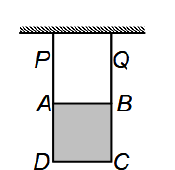
\includegraphics[width=0.35\linewidth]{Score-II - Test 29 (26 Mar 2024)-img/p1phy_n2_square.png}
\end{center}

\textbf{3.} In a hydrogen like atom an electron is orbiting in an orbit having quantum number n. Its frequency of revolution is found to be $13.2\times10^{15}$ Hz. Energy required to remove this electron from this orbit is 54.4 eV. In a time of 7 nano second the electron jumps back to orbit having quantum number $\dfrac n2$. $\tau$ (in Nm.) be the average torque acted on the electron during the above process, then find $\tau\times10^{27}$
(given: $\dfrac h\pi=2.1\times10^{-34}$ J-s, frequency of revolution of electron in the ground state of H-atom $v_0=6.6\times10^{15}$ Hz and ionization energy of H-atom, $E_0=13.6$ eV.

\textbf{4.} A small ball is projected from point P on floor towards a wall as shown. It hits the wall when its velocity is horizontal. Ball reaches point P after one bounce on the floor. If coefficient of restitution (e) is same for two collision find its value. Find $\dfrac1e$. Round off to nearest integer if necessary.

\begin{center}
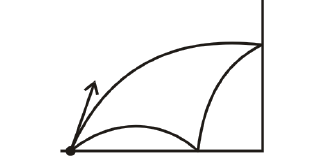
\includegraphics[width=0.5\linewidth]{Score-II - Test 29 (26 Mar 2024)-img/p1phy_n4_ball.png}
\end{center}

\textbf{5.} A small block is projected an a smooth horizontal surface terminating in a smooth quarter cylinder as shown. If the block losses contact at $\theta=\cos^{-1}\left(\dfrac45\right)$. What is initial velocity (in m/s)? (R = 1m)

\begin{center}
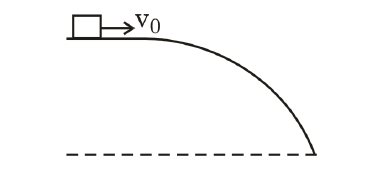
\includegraphics[width=0.5\linewidth]{Score-II - Test 29 (26 Mar 2024)-img/p1phy_n5_block.png}
\end{center}

\textbf{6.} A uniform rod of mass m, length $\ell$ and density $\rho$ is placed vertically with the lower end just touching the horizontal surface of a non-viscous and homogenous liquid of density $\sigma\ (\sigma<\rho)$ as shown. The rod is now released from rest. If the speed of the rod when half of its length is immersed in the liquid is $\sqrt{g\ell\left(1-\dfrac{\sigma}{n\rho}\right)}$, then find n.

\begin{center}
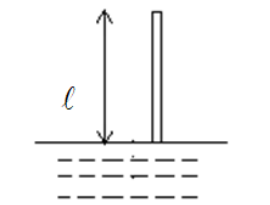
\includegraphics[width=0.4\linewidth]{Score-II - Test 29 (26 Mar 2024)-img/p1phy_n6_rod.png}
\end{center}

\sectionhdr{PART-2: CHEMISTRY}
\subsectionhdr{Section-I (i): Single Correct}

\textbf{1.} The value of $(n_2+n_1)$ and $(n_2^2-n_1^2)$ for He$^+$ ion in atomic spectrum are 4 and 8 respectively. The wavelength of emitted photon when electron jump from n$_2$ to n$_1$ is

\begin{qoptions}
\opt{A}{$\dfrac{32}{9}R_H$}
\opt{B}{$\dfrac{9}{32}R_H$}
\opt{C}{$\dfrac{9}{32R_H}$}
\opt{D}{$\dfrac{32}{9R_H}$}
\end{qoptions}

\textbf{2.} A$_3$B$_2$ is a sparingly soluble salt of molar mass M (g mole$^{-1}$) and solubility x g lit$^{-1}$. The ratio of the molar concentration of B$^{3-}$ to the solubility product of the salt is

\begin{qoptions}
\opt{A}{$108\dfrac{x^5}{M^5}$}
\opt{B}{$\dfrac1{108}\dfrac{M^4}{x^4}$}
\opt{C}{$\dfrac1{54}\dfrac{M^4}{x^4}$}
\opt{D}{None}
\end{qoptions}

\textbf{3.} Which one of the following statement is CORRECT?

\begin{qoptions}
\opt{A}{Ammonia gas can not be prepared by hydrolysis of calcium cyanamide}
\opt{B}{On heating ammonium nitrite, NH$_3$ gas is formed}
\opt{C}{On heating ammonium dichromate, laughing gas is formed}
\opt{D}{On heating ammonium carbonate, ammonia is formed}
\end{qoptions}

\textbf{4.} Product (C) is:

\begin{center}
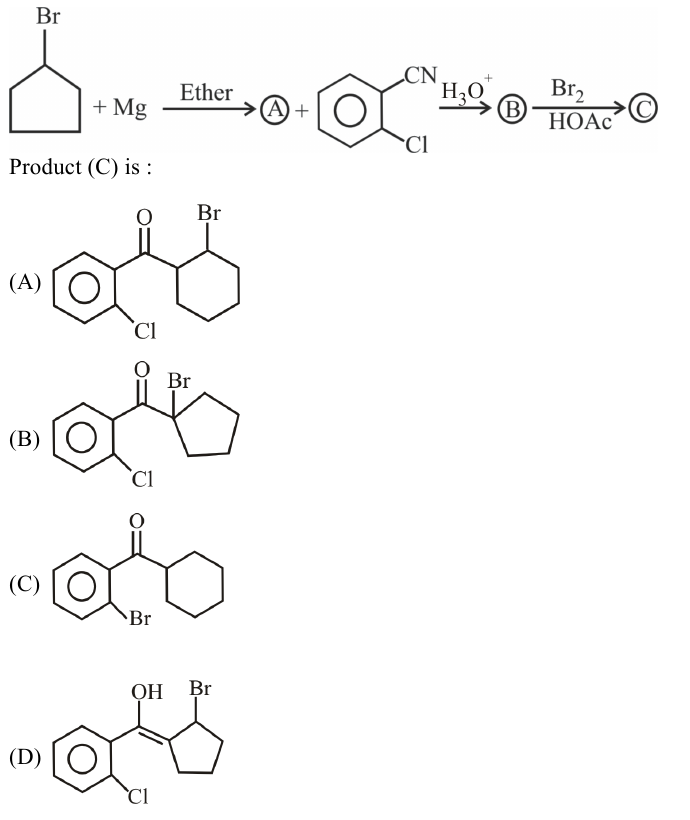
\includegraphics[width=0.95\linewidth]{Score-II - Test 29 (26 Mar 2024)-img/p2chem_q4_grignard.png}
\end{center}

\subsectionhdr{Section-I (ii): One or more correct}

\textbf{5.} Two volatile liquids A and B are mixed to form an ideal solution. If P$_A^o$ = 100mm of Hg \& P$_B^o$ = 150mm of Hg then identify the correct option(s) if 10 moles of A are mixed with 40 moles of B such that moles vaporised are very small.

\begin{qoptions}
\opt{A}{Total pressure when equilibrium gets established will be 140 mm of Hg.}
\opt{B}{Mole fraction of A in vapour state will be less than 0.5.}
\opt{C}{Mole fraction of B in vapour state is equal to $\dfrac67$}
\opt{D}{Moles of B in vapour state should be greater than 80\%}
\end{qoptions}

\textbf{6.} For the reaction,
A $\to$ Products (order = n)
the time of completion of reaction is

\begin{qoptions}
\opt{A}{Infinite for all value of `n'}
\opt{B}{Infinite for n = 1}
\opt{C}{$\dfrac{[A_0]^{1-n}}{K(1-n)}$ for n $\neq$ 1}
\opt{D}{$\dfrac{[A_0]^{1-n}}{K(1-n)}$ for n < 1}
\end{qoptions}

\textbf{7.} Which of the following statement is correct?

\begin{qoptions}
\opt{A}{The melting point of hydrides of Group 15 : NH$_3$ > SbH$_3$ > AsH$_3$ > PH$_3$}
\opt{B}{$\Delta H_{eg}$ kJ mol$^{-1}$ : S > Se > O > Te > Po}
\opt{C}{Melting point : B > Al > Tl > In > Ga}
\opt{D}{Bond enthalpy : C--C > Si--Si > Ge--Ge > Sn--Sn}
\end{qoptions}

\subsectionhdr{Section-I (iii): Matching List Sets}

\textbf{8.} Match the list:

\textbf{List-I}\\
(P) Isothermal reversible expansion of an ideal gas\\
(Q) Vapourisation of a liquid at its boiling point at 1 atm.\\
(R) Adiabatic reversible compression involving an ideal gas\\
(S) Combustion of CH$_4$ in sealed rigid adiabatic container.

\textbf{List-II}\\
(1) $\Delta S_{sys}=0$\quad (2) $\Delta U=0$\quad (3) $\Delta G=0$\quad (4) w = 0\quad (5) q = 0

\begin{qoptions}
\opt{A}{P $\to$ 1; Q $\to$ 4,2; R $\to$ 5; S $\to$ 3,4,5}
\opt{B}{P $\to$ 2; Q $\to$ 3; R $\to$ 1,5; S $\to$ 2,4,5}
\opt{C}{P $\to$ 2,3; Q $\to$ 1; R $\to$ 2; S $\to$ 1,2}
\opt{D}{P $\to$ 5; Q $\to$ 4,5; R $\to$ 1; S $\to$ 2}
\end{qoptions}

\textbf{9.} Match List-I with List-II:

\textbf{List-I}\\
(P) $[\text{Mn}(\text{H}_2\text{O})_6]^{2+}$\quad (Q) $[\text{Cr}(\text{H}_2\text{O})_6]^{3+}$\quad (R) $[\text{Fe}(\text{H}_2\text{O})_6]^{2+}$\quad (S) $[\text{Sc}(\text{H}_2\text{O})_6]^{3+}$

\textbf{List-II}\\
(1) Colourless\quad (2) Green\quad (3) Violet\quad (4) Pink\quad (5) Yellow

Choose the correct answer from the options given below:

\begin{qoptions}
\opt{A}{P $\to$ 3; Q $\to$ 5; R $\to$ 1; S $\to$ 3}
\opt{B}{P $\to$ 4; Q $\to$ 2; R $\to$ 3; S $\to$ 5}
\opt{C}{P $\to$ 4; Q $\to$ 3; R $\to$ 1; S $\to$ 2}
\opt{D}{P $\to$ 4; Q $\to$ 3; R $\to$ 2; S $\to$ 1}
\end{qoptions}

\textbf{10.} Match the particulars given in List (I) with the appropriate chemical reagents given in List (II).

\textbf{List-I}\\
(P) Fe$^{3+}$, Zn$^{2+}$ \& Cu$^{2+}$ can be distinguished by\\
(Q) PbS, CuS and CdS dissolve in\\
(R) Pb$^{2+}$ gives yellow precipitate with\\
(S) Bi$^{3+}$ gives a black precipitate with

\textbf{List-II}\\
(1) CsCl solution\quad (2) Alkaline Na$_2$SnO$_2$ solution\quad (3) 50\% HNO$_3$\quad (4) K$_2$CrO$_4$ solution\quad (5) Aqueous NH$_3$

\begin{qoptions}
\opt{A}{P $\to$ 5; Q $\to$ 3; R $\to$ 4; S $\to$ 2}
\opt{B}{P $\to$ 3; Q $\to$ 2; R $\to$ 4; S $\to$ 1}
\opt{C}{P $\to$ 2; Q $\to$ 4; R $\to$ 1; S $\to$ 3}
\opt{D}{P $\to$ 4; Q $\to$ 5; R $\to$ 2; S $\to$ 1}
\end{qoptions}

\textbf{11.}

\textbf{List-I}

(P)
\begin{center}
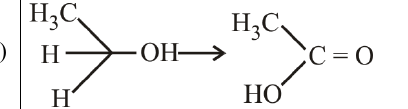
\includegraphics[width=0.9\linewidth]{Score-II - Test 29 (26 Mar 2024)-img/p2chem_q11_P.png}
\end{center}

(Q)
\begin{center}
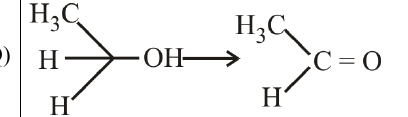
\includegraphics[width=0.9\linewidth]{Score-II - Test 29 (26 Mar 2024)-img/p2chem_q11_Q.png}
\end{center}

(R)
\begin{center}
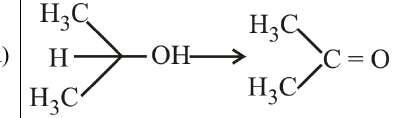
\includegraphics[width=0.9\linewidth]{Score-II - Test 29 (26 Mar 2024)-img/p2chem_q11_R.png}
\end{center}

(S)
\begin{center}
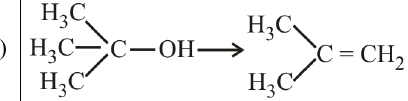
\includegraphics[width=0.9\linewidth]{Score-II - Test 29 (26 Mar 2024)-img/p2chem_q11_S.png}
\end{center}

\textbf{List-II}\\
(1) PCC (Pyridiumchlorochromate)\quad (2) Cu/573K\quad (3) K$_2$Cr$_2$O$_7$ + Dil H$_2$SO$_4$/293K\quad (4) KMnO$_4$, H$^+$/239K\quad (5) H$_3$PO$_4$/358K

\begin{qoptions}
\opt{A}{P $\to$ 3,4; Q $\to$ 1,2; R $\to$ 1,2,3,4; S $\to$ 2,5}
\opt{B}{P $\to$ 1,3; Q $\to$ 2,3,4; R $\to$ 4,5; S $\to$ 2,3}
\opt{C}{P $\to$ 2,3,4; Q $\to$ 4,5; R $\to$ 2,3; S $\to$ 1,2,3}
\opt{D}{P $\to$ 4,5; Q $\to$ 2,5; R $\to$ 1,2,3; S $\to$ 2,3,4}
\end{qoptions}

\subsectionhdr{Section-II: Numerical Value}

\textbf{1.} A metal `M' having atomic mass 31.25 crystallizes in cubic close packing and it show ``Schottky defects''. If the edge length of the cubic lattice is 500 pm and density of the metal 1.6075 gm/ml then calculate number of moles of metal atom `M' missing per litre of the crystal.
(Given: 1 amu = $1.67\times10^{-24}$ gm)

\textbf{2.} Na $\xrightarrow{\text{limited air}}$ X $\xrightarrow{\text{excess air}}$ Y

Choose the correct statement(s):-

(A) Oxidation state of oxygen is higher in `X' as compared to `Y'
(B) Both `X' and `Y' are diamagnetic
(C) `Y' on reaction with water produces H$_2$O$_2$
(D) Moist `X' on reaction with CO$_2$ produces Na$_2$CO$_3$
(E) Both X and Y are basic in nature
(F) X is soluble while Y is insoluble in nature.

\textbf{3.}

\begin{center}
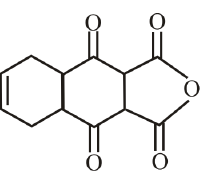
\includegraphics[width=0.35\linewidth]{Score-II - Test 29 (26 Mar 2024)-img/p2chem_n3_bicyclic.png}
\end{center}

$\xrightarrow[\text{(2) O}_3\quad\text{(3) H}_2\text{O}_2\quad\text{(4) }\Delta]{\text{(1) H}_3\text{O}^+,\,\Delta}$ Major product (A)

How many sp$^2$ carbon present in major product (A)?

\textbf{4.} For the given compound [x]. The total number of optical active stereoisomers are -

\begin{center}
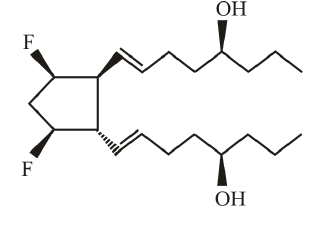
\includegraphics[width=0.75\linewidth]{Score-II - Test 29 (26 Mar 2024)-img/p2chem_n4_diene.png}
\end{center}

Where --
This type of bond indicate that the configuration at the specific carbon and the geometry of the double bond is fixed.
But this type of bond indicate that the configuration at the specific carbon and the geometry of the double bond in not fixed.

\textbf{5.} In the following reaction sequence. The compound [J] in an intermediate product

I $\xrightarrow[\text{CH}_3\text{COONa}]{\text{(CH}_3\text{CO)}_2\text{O}}$ J $\xrightarrow[\substack{\text{(2) Br}_2/\text{CCl}_4\\\text{(3) 2NaNH}_2\\\text{(4) HgSO}_4,\text{H}_2\text{SO}_4.\text{H}_2\text{O}\\\text{(5) NaOBr, H}_3\text{O}^+}]{\text{(1) NaOH, CaO, }\Delta}$ K + L $\xrightarrow[\substack{\text{(2) Br}_2,\text{KOH}\\\text{(3) (CH}_3\text{CO)}_2\text{O, pyridine}}]{\text{(1) NH}_3,\,\Delta}$ M

What is the degree of unsaturation of M?

\textbf{6.} The sum of geometrical isomers in [Pt(H$_2$N--CH(CH$_3$)COO$^-$)$_2$] complex and stereoisomers of [Pt(gly)$_3$]$^+$ complex is \_\_\_\_\_\_\_\_.

\sectionhdr{PART-3: MATHEMATICS}
\subsectionhdr{Section-I (i): Single Correct}

\textbf{1.} Given three points on the x-y plane of O(0,0), A(1,0) and B($-1$,0). Point P is moving on the plane satisfying the condition $(\overrightarrow{PA}.\overrightarrow{PB})+3(\overrightarrow{OA}.\overrightarrow{OB})=0$. If the maximum and minimum values of $|\overrightarrow{PA}||\overrightarrow{PB}|$ are M and m, respectively then find the value of M$^2$+m$^2$

\begin{qoptions}
\opt{A}{24}
\opt{B}{34}
\opt{C}{44}
\opt{D}{None of these}
\end{qoptions}

\textbf{2.} If $\displaystyle\lim_{x\to k^-}[\sin^{-1}x+\cos^{-1}x+\tan^{-1}x]$ does not exist, then sum of the all possible values of k is.
[Note: [y] denotes greatest integer function less than or equal to y.]

\begin{qoptions}
\opt{A}{$\dfrac{-\sin3}{\sin1\cdot\sin2}$}
\opt{B}{$\dfrac{-\sin2}{\sin1\cdot\sin3}$}
\opt{C}{$\dfrac{-\sin1}{\sin2\cdot\sin3}$}
\opt{D}{$\dfrac{-\sin1\cdot\sin2}{\sin3}$}
\end{qoptions}

\textbf{3.} The mean of five observations is 4 and their variance is 5.2. It three of these observation are 1, 2 and 6 then the other two are

\begin{qoptions}
\opt{A}{2 and 9}
\opt{B}{3 and 8}
\opt{C}{4 and 7}
\opt{D}{5 and 6}
\end{qoptions}

\textbf{4.} Let $f'(\sin x)<0$ and $f''(\sin x)>0,\ \forall x\in\left(0,\dfrac\pi2\right)$ and $g(x)=f(\sin x)+f(\cos x)$, then g(x) is decreasing in

\begin{qoptions}
\opt{A}{$\left(\dfrac\pi4,\dfrac\pi2\right)$}
\opt{B}{$\left(0,\dfrac\pi4\right)$}
\opt{C}{$\left(0,\dfrac\pi2\right)$}
\opt{D}{$\left(\dfrac\pi6,\dfrac\pi2\right)$}
\end{qoptions}

\subsectionhdr{Section-I (ii): One or more correct}

\textbf{5.} Let $X=\displaystyle\sum_{r=0}^n\left(\dfrac{(-1)^r}{r+1}\right)$, then $|X-\ln2|$, will be -

\begin{qoptions}
\opt{A}{greater than $\dfrac1{2(n+1)}$}
\opt{B}{greater than $\dfrac1{2(n+2)}$}
\opt{C}{less than $\dfrac1{2(n+1)}$}
\opt{D}{less than $\dfrac1{2(n+2)}$}
\end{qoptions}

\textbf{6.} Let M denote the matrix $\begin{pmatrix}0&i\\i&0\end{pmatrix}$, where $i^2=-1$, and let I denote the identity matrix $\begin{pmatrix}1&0\\0&1\end{pmatrix}$
Then the matrix $I+M+M^2+M^3+M^4+\ldots\ldots+M^{2010}$ is equal to

\begin{qoptions}
\opt{A}{$\begin{pmatrix}0&0\\0&0\end{pmatrix}$}
\opt{B}{$\begin{pmatrix}0&i\\i&0\end{pmatrix}$}
\opt{C}{$\begin{pmatrix}1&i\\i&1\end{pmatrix}$}
\opt{D}{$\begin{pmatrix}-1&0\\0&-1\end{pmatrix}$}
\end{qoptions}

\textbf{7.} Let $z_1,z_2,z_3\in\mathbb C$ such that $|z_1|=1$, $|z_2-(1+\sqrt3 i)|=3$, and $|z_3-3-3\sqrt3 i|=7$. If $|3z_1-2z_2-4z_3|$ is maximum then

\begin{qoptions}
\opt{A}{maximum value of $|z_1-z_2|=5$}
\opt{B}{maximum value of $|z_3-z_1|=14$}
\opt{C}{$|z_1|+|z_2|+|z_3|=17$}
\opt{D}{$z_3+3z_1=2z_2$}
\end{qoptions}

\subsectionhdr{Section-I (iii): Matching List Sets}

\textbf{8.} Let $f(x)=2\sin^2\beta+4\cos(x+\beta)\sin x\sin\beta+\cos2(x+\beta)$ and $g(x)=\left(\displaystyle\lim_{\alpha\to0}(1+\alpha)^{1/\alpha}\right)^{\tan(\tan^{-1}x)}$ then

\textbf{List-I}\\
(P) If $\displaystyle\lim_{x\to0}(f(x))^{1/x^2}=\ell$ then $2\ell n\,\ell^{-1}$ is equal to\\
(Q) $\displaystyle\lim_{x\to0}\dfrac{g(x)-f(x)}{2x}$ is equal to\\
(R) If x $\in(-\infty,0]$ then number of integer(s) in the range of h(x) = 1 + g(x) is(are)\\
(S) The number of solution(s) of the equation $f(x)=\dfrac12$ in [0,3] is/are

\textbf{List-II}\\
(1) $\dfrac12$\quad (2) 1\quad (3) 2\quad (4) 4\quad (5) 5

\begin{qoptions}
\opt{A}{P $\to$ 1; Q $\to$ 4; R $\to$ 5; S $\to$ 2}
\opt{B}{P $\to$ 4; Q $\to$ 1; R $\to$ 2; S $\to$ 3}
\opt{C}{P $\to$ 2; Q $\to$ 5; R $\to$ 4; S $\to$ 1}
\opt{D}{P $\to$ 3; Q $\to$ 2; R $\to$ 1; S $\to$ 5}
\end{qoptions}

\textbf{9.}

\textbf{List-I}\\
(P) An equilateral triangle has one vertex at (0,0) and another at $(3,\sqrt3)$ the x-coordinate of third vertex is\\
(Q) $(1,-2)$, $(3,6)$, $(5,10)$, $(3,y)$ in order are the vertices of a parallelogram, then y is\\
(R) x-coordinate of circumcentre of triangle with vertices $(-2,-3)$, $(-1,0)$, $(7,-6)$ is\\
(S) y-coordinate of a point which divides the line segment joining $(5,-2)$ and $(9,6)$ internally in the ratio 3 : 1, is

\textbf{List-II}\\
(1) 5\quad (2) 1\quad (3) 2\quad (4) 3\quad (5) 4

\begin{qoptions}
\opt{A}{P $\to$ 5; Q $\to$ 4; R $\to$ 3; S $\to$ 2}
\opt{B}{P $\to$ 2; Q $\to$ 1; R $\to$ 4; S $\to$ 3}
\opt{C}{P $\to$ 3; Q $\to$ 4; R $\to$ 1; S $\to$ 2}
\opt{D}{P $\to$ 4; Q $\to$ 3; R $\to$ 4; S $\to$ 5}
\end{qoptions}

\textbf{10.} In the adjoining figure

\begin{center}
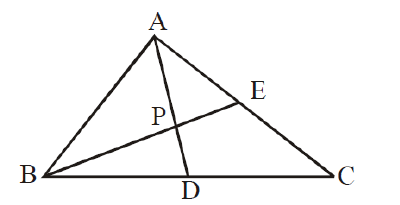
\includegraphics[width=0.55\linewidth]{Score-II - Test 29 (26 Mar 2024)-img/p3math_q10_triangle.png}
\end{center}

BD : DC = 3 : 4,
BP : PE = $\sin2\theta$ : $\cos\theta$ \& E is the mid point of AC.

\textbf{List-I}\\
(P) Value of $\left[\dfrac{AP}{PD}\right]$ is (where [.] denotes greatest integer function)\\
(Q) Number of values of $\theta\in[0,4\pi]$ is\\
(R) If $\lambda(\overrightarrow{BA}+\overrightarrow{BC})=10\overrightarrow{BP}$, then $\lambda$ is\\
(S) Value of $\left[\dfrac{BP}{PE}\right]$ is (where [.] denotes greatest integer function)

\textbf{List-II}\\
(1) 3\quad (2) 2\quad (3) 1\quad (4) 4\quad (5) 6

\begin{qoptions}
\opt{A}{P $\to$ 3; Q $\to$ 1; R $\to$ 5; S $\to$ 2}
\opt{B}{P $\to$ 1; Q $\to$ 2; R $\to$ 3; S $\to$ 5}
\opt{C}{P $\to$ 2; Q $\to$ 4; R $\to$ 1; S $\to$ 3}
\opt{D}{P $\to$ 4; Q $\to$ 3; R $\to$ 5; S $\to$ 4}
\end{qoptions}

\textbf{11.} Let $f(x)=(\ell n(a^2-3a-3))|\sin x|+\left[\dfrac{a^2}9\right]\cos\pi x\ \forall x\in\mathbb R,\ a\in[-4,4]$
(where [ ] denotes greatest integer function)

\textbf{List-I}\\
(P) If f(x) is periodic then the number of integral values of a is\\
(Q) If f(x) is periodic with period to be a rational number then number of integral values of a is\\
(R) If f(x) is periodic with period to be an irrational then number of integral values of a is\\
(S) If f(x) is non periodic function then number of integral values of a is

\textbf{List-II}\\
(1) 1\quad (2) 2\quad (3) 3\quad (4) 4\quad (5) 5

\begin{qoptions}
\opt{A}{P $\to$ 2; Q $\to$ 1; R $\to$ 3; S $\to$ 4}
\opt{B}{P $\to$ 3; Q $\to$ 1; R $\to$ 1; S $\to$ 2}
\opt{C}{P $\to$ 5; Q $\to$ 3; R $\to$ 1; S $\to$ 4}
\opt{D}{P $\to$ 5; Q $\to$ 1; R $\to$ 3; S $\to$ 4}
\end{qoptions}

\subsectionhdr{Section-II: Numerical Value}

\textbf{1.} If the two lines AB : $\left(\displaystyle\int_0^{2t}\left(\dfrac{\sin x}{x}+1\right)dx\right)x+y=3t$ and AC : $2tx+y=0$ intersect at a point A, then x-coordinate of point A as $t\to0$, is equal to $\dfrac pq$ (p and q are in their lowest form). Then (p + q) is

\textbf{2.} Let A$_1$, A$_2$, A$_3$, A$_4$ be the areas of the triangular faces of a tetrahedron, and h$_1$, h$_2$, h$_3$, h$_4$ be the corresponding altitudes of the tetrahedron. If volume of tetrahedron is 5 cubic units, then the minimum value of $\dfrac{(A_1+A_2+A_3+A_4)(h_1+h_2+h_3+h_4)}{60}$ (in cubic units) is

\textbf{3.} Let $z_1,z_2,z_3$ be complex numbers such that $z_1^2+z_2^2+z_3^2=z_1z_2+z_2z_3+z_3z_1$ and $|z_1+z_2+z_3|=21$. Given that $|z_1-z_2|=2\sqrt3$, $|z_1|=3\sqrt3$. Compute $|z_2|^2+|z_3|^2$.

\textbf{4.} If the value of $\displaystyle\lim_{n\to\infty}(n^3+n^2)^{1/3}-\left[\sqrt{{}^{(n+1)}P_2}\right]=\dfrac pq$, where n $\in$ N then find the value of (p + q).
[Note: [y] denotes greatest integer function less than or equal of y.]

\textbf{5.} Let f(x) be a polynomial satisfies the relation $f(f(f(x)))+(1-p)f(x)=3,\ \forall x\in\mathbb R$, where p is any real number. If leading coefficient of f(x) is 2 then find the value of $\left(\dfrac{d}{dx}f(f(x))\text{ at }x=p\right)+\displaystyle\int_{-p}^p(2f^{-1}(x)+1)\,dx$.

\textbf{6.} Let $f(x)=\dfrac{\sin^{-1}x+\tan^{-1}x-\cos^{-1}x-\cot^{-1}x}{\sin^{-1}x+\tan^{-1}x+\cos^{-1}x+\cot^{-1}x}$. If the maximum and minimum value of f(x) is M and m respectively, then find the value of $9M-m+\displaystyle\sum_{k=0}^\infty M^k$.

\end{document}
